\begin{figure}
\centering
\begin{subfigure}[t]{0.48\textwidth}
\begin{center}
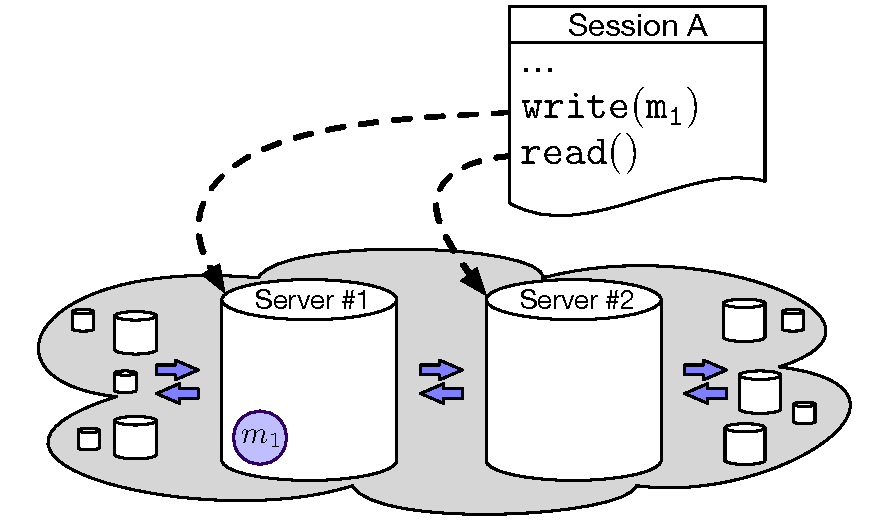
\includegraphics[scale=0.45]{../Figures/System_example.pdf}
\end{center}
\label{fig:rmw_falsified} \vspace{0 mm}
\caption{ $\mathtt{read}$ operation is sent to server\#2 that does not yet
contain $m_1$, a message previously submitted by the same session}
\end{subfigure}\quad
\begin{subfigure}[t]{0.48\textwidth}
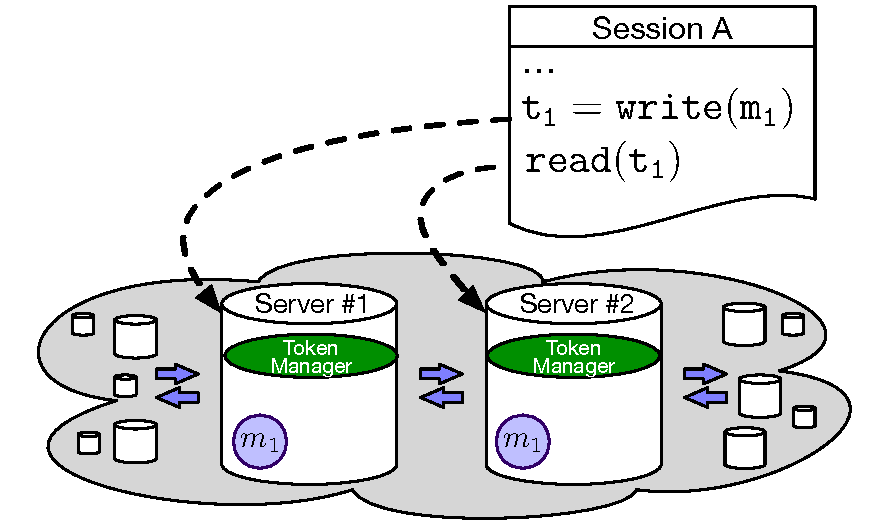
\includegraphics[scale=0.45]{../Figures/System_example_adhoc.pdf}
\label{fig:addhoc_impl}
\caption{Each $\mathtt{write}$ is responded with a token, which is later
passed with each $\mathtt{read}$. The token manager at the server side,
blocks the read requests, until the desired token is available, which
here means that $m_1$ has arrived. }
\end{subfigure}
\\ \hrulefill 
\caption {A behavior allowed under eventual consistency, that
falsifies RMW (left).  Ad-hoc modification of the application to
maintain RMW (right)}


\end{figure}

